\documentclass[a4paper,11pt,exos]{nsi} % COMPILE WITH DRAFT
\usepackage{pifont}
\usepackage{fontawesome5}
\usepackage{hyperref}
\usepackage{pgfplots}


\begin{document}
\classe{\terminale Comp}
\titre{Corrigés des execices - Chap 5}
\maketitle

\subsection*{Vérifier qu’une fonction donnée est solution d’une équation différentielle.}

\begin{methode}
Pour vérifier qu'une fonction $f$ est solution d'une équation différentielle du premier ordre :
\begin{enumerate}[label=\bullet]
    \item On calcule $f'$ ;
    \item On évalue séparemment les deux membres de l'équation différentielle en remplaçant $f(x)$ et $f'(x)$ par leurs expressions ;
    \item On vérifie que les deux membres de l'égalité sont égaux.
\end{enumerate}
\end{methode}
\exo{}
On considère l'équation différentielle $y' = 2x+1$ pour $x$ réel.\\
Montrer que la fonction $f$ définie sur $\R$ par $f(x)=x^2+x+3$ est solution de cette équation différentielle.\\

\textcolor{UGLiBlue}{
    Soit $f$ la fonction définie sur $\R$ par $f(x)=x^2+x+3$.\\
    On a : pour tout $x\in\R, \quad f'(x)=2x+1$.\\
    Donc $f$ est solution de l'équation différentielle $y'=2x+1$.
}

\exo{}
On considère l'équation différentielle $y'-2y = 0$.\\
Montrer que la fonction $g$ définie sur $\R$ par $g(x)=e^{2x}$ est solution de cette équation différentielle.\\

\textcolor{UGLiBlue}{
    Soit $g$ la fonction définie sur $\R$ par $g(x)=e^{2x}$.\\
    On a : pour tout $x\in\R, \quad g'(x)=2e^{2x}$.
    \begin{tabbing}
       Donc $\quad g'(x)-2g(x)$ \= $= 2e^{2x}-2e^{2x}$\\
        \>  $=0$.
    \end{tabbing}
    Donc $g$ est solution de l'équation différentielle $y'-2y=0$.
}

\exo{}
On considère l'équation différentielle $xy'+y = x$ pour $x$ réel.\\
Montrer que la fonction $h$ définie sur $\R$ par $h(x)=\dfrac{1}{2}x$ est solution de cette équation différentielle.\\

\textcolor{UGLiBlue}{
    Soit $h$ la fonction définie sur $\R$ par $h(x)=\dfrac{1}{2}x$.\\
    On a : pour tout $x\in\R : \quad h'(x)=\dfrac{1}{2}$.
    \begin{tabbing}
        Donc $\quad xh'(x)+h(x)$ \= $= x\times\dfrac{1}{2}+\dfrac{1}{2}x$\\
        \> $=\dfrac{1}{2}x+\dfrac{1}{2}x$\\
        \> $=x$.
    \end{tabbing}
    Donc $h$ est solution de l'équation différentielle $xy'+y=x$.
}

\exo{}
On considère l'équation différentielle $(E) : y' = 2+e^{-x}$ pour $x$ réel.\\
Dans chaque cas, vérifier si la fonction définie sur $\R$ est solution de $(E)$ :
\begin{multicols}{2}
    \begin{enumerate}
        \item $f:x\mapsto 2x+e^{-x}$
        \item $g:x\mapsto \dfrac{2xe^x+1}{e^x}$
    \end{enumerate}
\end{multicols}

\textcolor{UGLiBlue}{
    \begin{enumerate}
        \item Soit $f$ la fonction définie sur $\R$ par $f(x)=2x+e^{-x}$.\\
        On a : pour
        tout $x\in\R, \quad f'(x)=2-e^{-x}$.\\
        Donc $f$ n'est pas solution de l'équation différentielle $y'=2+e^{-x}$.
        \item Soit $g$ la fonction définie sur $\R$ par $g(x)=\dfrac{u(x)}{v(x)}$.
        \begin{tabbing}
            Avec, pour tout $x\in\R$ $\quad$ \=$u(x)=2xe^x+1\qquad$ \= et $\qquad$ \=$ v(x)=e^x$\\
            \> $u'(x)=2e^x+2xe^x$ \> et \> $v'(x)=e^x$\\[1em]
            Donc, pour tout $x\in\R$ \> $g'(x)=\dfrac{u'(x)v(x)-u(x)v'(x)}{v(x)^2}$\\[.5em]
            \> $\phantom{g'(x)}=\dfrac{(2e^x+2xe^x)e^x-(2xe^x+1)e^x}{e^{2x}}$\\[.5em]
            \> $\phantom{g'(x)}=\dfrac{2e^{2x}+2xe^{2x}-2xe^{2x}-e^{x}}{e^{2x}}$\\[.5em]
            \> $\phantom{g'(x)}=\dfrac{2e^{2x}-e^x}{e^{2x}}$\\[.5em]
            \> $\phantom{g'(x)}=2+\dfrac{1}{e^x}$\\[.5em]
            \> $\phantom{g'(x)}=2+e^{-x}$.
        \end{tabbing}
        Donc $g$ est solution de l'équation différentielle $y'=2+e^{-x}$.
    \end{enumerate}
}

\subsection*{Vérifier qu'une fonction est une primitive d'une fonction donnée.}

\begin{methode}
Pour vérifier qu'une fonction $F$ est une primitive d'une fonction $f$ donnée, on dérive $F$ et on vérifie que $F'=f$.
\end{methode}

\exo{}
Soient $f$ et $F$ les fonctions définies sur $\R$ par $f(x)= xe^x$ et $F(x)= (x-1)e^x$.
\begin{enumerate}
    \item Montrer que $F$ est une primitive de $f$ sur $\R$.
    \item En déduire toutes les primitives de $f$ sur $\R$.
\end{enumerate}

\textcolor{UGLiBlue}{
    \begin{enumerate}
        \item Soit $F$ la fonction définie sur $\R$ par $F(x)=(x-1)e^x$.
        \begin{tabbing}
            On a : pour tout $x\in\R, \quad F'(x)$  \=$=e^x+(x-1)e^x$\\
            \> $=e^x+xe^x-e^x$\\
            \> $=xe^x$\\
            \> $=f(x)$.
        \end{tabbing}
        Donc $F$ est une primitive de $f$ sur $\R$.
        \item Donc toutes les primitives de $f$ sur $\R$ sont les fonctions définies sur $\R$ par $x\mapsto (x-1)e^x+C$ où $C$ est une constante réelle.
    \end{enumerate}
}

\exo{}
Soient $f$ et $F$ les fonctions définies sur $\oio{0}{+\infty}$ par $f(x)= \dfrac{2x+3}{x}$ et $F(x)=2x+3\ln(x)$.
\begin{enumerate}
    \item Montrer que $F$ est une primitive de $f$ sur $\oio{0}{+\infty}$.
    \item Déterminer la primitive de $f$ sur $\oio{0}{+\infty}$ qui s'annule en $1$.
\end{enumerate}

\textcolor{UGLiBlue}{
    \begin{enumerate}
        \item Soit $F$ la fonction définie sur $\oio{0}{+\infty}$ par $F(x)=2x+3\ln(x)$.
        \begin{tabbing}
            On a : pour tout $x\in\oio{0}{+\infty}, \quad F'(x)$ \= $=2+\dfrac{3}{x}$\\
            \> $=\dfrac{2x+3}{x}$\\
            \> $=f(x)$.
        \end{tabbing}
        Donc $F$ est une primitive de $f$ sur $\oio{0}{+\infty}$.
        \item La primitive de $f$ sur $\oio{0}{+\infty}$ qui s'annule en $1$ est la fonction définie sur $\oio{0}{+\infty}$ par $x\mapsto 2x+3\ln(x)-3$.
    \end{enumerate}
}

\newpage

\subsection*{Calculer un primitive en utilisant les fonctions de référence}
\exo{}
Dans chaque cas, déterminer une primitive sur $I$ de la fonction définie :
\begin{multicols}{2}
    \begin{enumerate}
        \item $f(x)=x^2-6x+5, \qquad I=\R$
        \item $g(x)=5x^3+4x^2-x+1, \qquad I=\R$
        \item $h(x)=7x^3-\dfrac{3}{x}, \qquad I=\oio{0}{+\infty}$
        \item $k(x)=\dfrac{1}{4}e^x+2x, \qquad I=\R$
        \item $l(x)=\dfrac{2}{x}+5e^x, \qquad I=\oio{0}{+\infty}$
        \item $m(x)=\dfrac{1}{x^2}-3x^2, \qquad I=\oio{0}{+\infty}$
    \end{enumerate}
\end{multicols}

\textcolor{UGLiBlue}{
    \begin{enumerate}
        \item Une primitive de $f$ sur $\R$ est la fonction $F$ définie sur $\R$ par $F(x)=\dfrac{1}{3}x^3-3x^2+5x$.
        \item Une primitive de $g$ sur $\R$ est la fonction $G$ définie sur $\R$ par $G(x)=\dfrac{5}{4}x^4+\dfrac{4}{3}x^3-\dfrac{1}{2}x^2+x$.
        \item Une primitive de $h$ sur $\oio{0}{+\infty}$ est la fonction $H$ définie sur $\oio{0}{+\infty}$ par $H(x)=\dfrac{7}{4}x^4-3\ln(x)$.
        \item Une primitive de $k$ sur $\R$ est la fonction $K$ définie sur $\R$ par $K(x)=\dfrac{1}{4}e^x+x^2$.
        \item Une primitive de $l$ sur $\oio{0}{+\infty}$ est la fonction $L$ définie sur $\oio{0}{+\infty}$ par $L(x)=2\ln(x)+5e^x$.
        \item Une primitive de $m$ sur $\oio{0}{+\infty}$ est la fonction $M$ définie sur $\oio{0}{+\infty}$ par $M(x)=-\dfrac{1}{x}+x^3$.
    \end{enumerate}
}

\subsection*{Déterminer d'autres primitives}

\exo{}
Déterminer une primitive de chacune des fonctions suivantes sur l'intervalle $I$.
\begin{enumerate}
    \item $f:x\mapsto -e^{-x}, \quad I=\R$
    \item $g:x\mapsto \dfrac{3x^2}{x^3+5}, \quad I=\oio{0}{+\infty}$
    \item $h:x\mapsto 2(2x+1)(x^2+x-7), \quad I=\R$
\end{enumerate}

\textcolor{UGLiBlue}{
    \begin{enumerate}
        \item Pour $x\in\R, f(x)=u'(x)e^{u(x)}\quad$ avec $\quad u(x)=-x\quad$ et $\quad u'(x)=-1$.\\
        Donc une primitive de $f$ sur $\R$ est la fonction $F$ définie sur $\R$ par $F(x)=e^{-x}$.
        \item Pour $x\in\oio{0}{+\infty}, g(x)=\dfrac{u'(x)}{u(x)}\quad$ avec $\quad u(x)=x^3+5>0\quad$ et $\quad u'(x)=3x^2$.\\
        Donc une primitive de $g$ sur $\oio{0}{+\infty}$ est la fonction $G$ définie sur $\oio{0}{+\infty}$ par $G(x)=\ln(x^3+5)$.
        \item Pour $x\in\R, h(x)=2u'(x)u(x)\quad$ avec $\quad u(x)=x^2+x-7\quad$ et $\quad u'(x)=2x+1$.\\
        Donc une primitive de $h$ sur $\R$ est la fonction $H$ définie sur $\R$ par $H(x)=(x^2+x-7)^2$.
    \end{enumerate}
}
       
\exo{}
Déterminer une primitive de chacune des fonctions suivantes sur l'intervalle $I$.
%\begin{multicols}{3}
    \begin{enumerate}
        \item $f:x\mapsto 2(3x^2+2)(x^3+2x), \quad I=\R$
        \item $g:x\mapsto (2x+1)e^{x^2+x+2}, \quad I=\R$
        \item $h:x\mapsto \dfrac{2x}{x^2+1}, \quad I=\R$
    \end{enumerate}
%\end{multicols}

\textcolor{UGLiBlue}{
    \begin{enumerate}
        \item Pour $x\in\R, f(x)=2u'(x)u(x)\quad$ avec $\quad u(x)=x^3+2x\quad$ et $\quad u'(x)=3x^2+2$.\\
        Donc une primitive de $f$ sur $\R$ est la fonction $F$ définie sur $\R$ par $F(x)=\left(x^3+2x\right)^2$.
        \item Pour $x\in\R, g(x)=u'(x)e^{u(x)}\quad$ avec $\quad u(x)=x^2+x+2\quad$ et $\quad u'(x)=2x+1$.\\
        Donc une primitive de $g$ sur $\R$ est la fonction $G$ définie sur $\R$ par $G(x)=e^{x^2+x+2}$.
        \item Pour $x\in\R, h(x)=\dfrac{u'(x)}{u(x)}\quad$ avec $\quad u(x)=x^2+1>0\quad$ et $\quad u'(x)=2x$.\\
        Donc une primitive de $h$ sur $\R$ est la fonction $H$ définie sur $\R$ par $H(x)=\ln(x^2+1)$.
    \end{enumerate}
}

\exo{}
Déterminer une primitive de chacune des fonctions suivantes sur l'intervalle $I$.
\begin{enumerate}
    \item $f:x\mapsto 2(4x^3+3)(x^4+3x), \quad I=\R$
    \item $g:x\mapsto \dfrac{3}{3x-1}, \quad I=\oio{\dfrac{1}{3}}{+\infty}$
    \item $h:x\mapsto 2e^{2x+1}, \quad I=\R$
\end{enumerate}

\textcolor{UGLiBlue}{
    \begin{enumerate}
        \item Pour $x\in\R, f(x)=2u'(x)u(x)\quad$ avec $\quad u(x)=x^4+3x\quad$ et $\quad u'(x)=4x^3+3$.\\
        Donc une primitive de $f$ sur $\R$ est la fonction $F$ définie sur $\R$ par $F(x)=\left(x^4+3x\right)^2$.
        \item Pour $x\in\oio{\dfrac{1}{3}}{+\infty}, g(x)=\dfrac{u'(x)}{u(x)}\quad$ avec $\quad u(x)=3x-1>0\quad$ et $\quad u'(x)=3$.\\
        Donc une primitive de $g$ sur $\oio{\dfrac{1}{3}}{+\infty}$ est la fonction $G$ définie sur $\oio{\dfrac{1}{3}}{+\infty}$ par $G(x)=\ln(3x-1)$.
        \item Pour $x\in\R, h(x)=u'(x)e^{u(x)}\quad$ avec $\quad u(x)=2x+1\quad$ et $\quad u'(x)=2$.\\
        Donc une primitive de $h$ sur $\R$ est la fonction $H$ définie sur $\R$ par $H(x)=e^{2x+1}$.
    \end{enumerate}
}

\newpage

\subsection*{Résoudre une équation différentielle de la forme $y'=ay$}
\exo{}
\begin{enumerate}
    \item Résoudre l'équation différentielle $3y'=2y$.
    \item Donner l'allure des courbes représentatives des solutions de cette équation différentielle.
    \item Déterminer l'unique solution $f$ de cette équation différentielle qui vérifie $f(1)=e$.
\end{enumerate}

\textcolor{UGLiBlue}{
    \begin{enumerate}
        \item L'équation différentielle $3y'=2y$ est équivalente à $y'=\dfrac{2}{3}y$.\\
        C'est une équation différentielle de la forme $y'=ay$ avec $a=\dfrac{2}{3}$.\\
        Les solutions de cette équation différentielle sont les fonctions définies sur $\R$ par $x\mapsto ke^{\frac{2}{3}x}$ où $k$ est une constante réelle.
        \item Allure des courbes représentatives des solutions de cette équation différentielle :
        \begin{center}
            \begin{tikzpicture}
                \begin{axis}[
                    axis lines = middle,
                    domain = -2:2,
                    samples = 100,
                    width = 8cm,
                    height = 8cm,
                    xtick=\empty,
                    ytick=\empty,
                    minor tick num = 5,
                    enlargelimits = true,
                    legend pos = north west,
                ]
                \addplot[
                    thick,
                    UGLiGreen,
                ]
                {2*exp(x)};
                \addlegendentry[UGLiGreen]{$k>0$}
                \addplot[
                    thick,
                    UGLiOrange,
                ]
                {-2*exp(x)};
                \addlegendentry[UGLiOrange]{$k<0$}
                \end{axis}
            \end{tikzpicture}
        \end{center}
        \item Soient $k$ une constante réelle et $f$ la fonction définie sur $\R$ par $f(x)=ke^{\frac{2}{3}x}$.
        \begin{tabbing}
            $f(1)=e\quad$ \= $\iff \quad ke^{\frac{2}{3}}=e$\\
            \> $\iff \quad k=e\times e^{-\frac{2}{3}}$\\
            \> $\iff \quad k=e^{\frac{1}{3}}$.
        \end{tabbing}
        Donc l'unique solution de cette équation différentielle qui vérifie $f(1)=e$ est la fonction définie sur $\R$ par $f(x)= e^{\frac{1}{3}}e^{\frac{2}{3}x}=e^{\frac{1}{3}+\frac{2}{3}x}$.
    \end{enumerate}
}



\exo{}
\begin{enumerate}
    \item Résoudre les équations différentielles :
    \begin{multicols}{2}
        \begin{enumalph}
            \item $y'=2y$
            \item $y'=-5y$
        \end{enumalph}
    \end{multicols}
    \item Donner l'allure des courbes représentatives des fonctions $x\mapsto K e^{-5x}$ suivant le signe du réel $K$.
\end{enumerate}

\textcolor{UGLiBlue}{
    \begin{enumerate}
        \item 
            \begin{enumalph}
                \item L'équation différentielle $y'=2y$ est de la forme $y'=ay$ avec $a=2$.\\
                Les solutions de cette équation différentielle sont les fonctions définies sur $\R$ par $x\mapsto ke^{2x}$ où $k$ est une constante réelle.
                \item L'équation différentielle $y'=-5y$ est de la forme $y'=ay$ avec $a=-5$.\\
                Les solutions de cette équation différentielle sont les fonctions définies sur $\R$ par $x\mapsto ke^{-5x}$ où $k$ est une constante réelle.
            \end{enumalph}
        \item Allure des courbes représentatives des solutions de ces équations différentielles :
        \begin{multicols}{2}
            \begin{enumalph}
                \item \begin{tikzpicture}
                    \begin{axis}[
                        axis lines = middle,
                        domain = -2:2,
                        samples = 100,
                        width = 8cm,
                        height = 8cm,
                        xtick=\empty,
                        ytick=\empty,
                        minor tick num = 5,
                        enlargelimits = true,
                        legend pos = north west,
                    ]
                    \addplot[
                        thick,
                        UGLiGreen,
                    ]
                    {2*exp(x)};
                    \addlegendentry[UGLiGreen]{$k>0$}
                    \addplot[
                        thick,
                        UGLiOrange,
                    ]
                    {-2*exp(x)};
                    \addlegendentry[UGLiOrange]{$k<0$}
                    \end{axis}
                \end{tikzpicture}
                \item \begin{tikzpicture}
                    \begin{axis}[
                        axis lines = middle,
                        domain = -2:2,
                        samples = 100,
                        width = 8cm,
                        height = 8cm,
                        xtick=\empty,
                        ytick=\empty,
                        minor tick num = 5,
                        enlargelimits = true,
                        legend pos = north east,
                    ]
                    \addplot[
                        thick,
                        UGLiGreen,
                    ]
                    {200*exp(-2*x)};
                    \addlegendentry[UGLiGreen]{$k>0$}
                    \addplot[
                        thick,
                        UGLiOrange,
                    ]
                    {-200*exp(-2*x)};
                    \addlegendentry[UGLiOrange]{$k<0$}
                    \end{axis}
                \end{tikzpicture}
            \end{enumalph}
        \end{multicols}
    \end{enumerate}
}

\dleft{11.5cm}{
    \exo{}
    Parmi les courbes suivantes, quelle est celle qui correspond à la solution de l'équation différentielle $y'+y=0$ qui prend la valeur $\dfrac{1}{2}$ en $0$ ?
}
{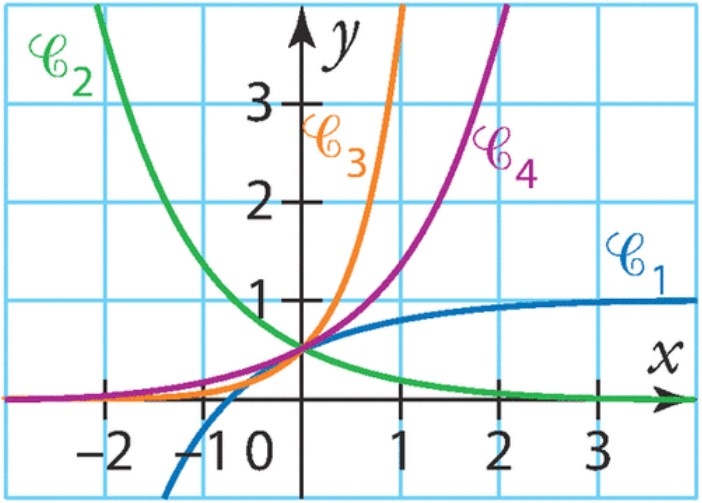
\includegraphics[width=5cm]{courbes1.jpg}}

\textcolor{UGLiBlue}{
    L'équation différentielle $y'+y=0$ est équivalente à $y'=-y$.\\
    C'est une équation différentielle de la forme $y'=-ay$ avec $a=1$.\\
    Les solutions de cette équation différentielle sont les fonctions définies sur $\R$ par $x\mapsto ke^{-x}$ où $k$ est une constante réelle.\\
    Elle est représentée graphiquement par une courbe d'allure :
    \begin{center}
        \begin{tikzpicture}
            \begin{axis}[
                axis lines = middle,
                domain = -2:2,
                samples = 100,
                width = 8cm,
                height = 6cm,
                xtick=\empty,
                ytick=\empty,
                minor tick num = 5,
                enlargelimits = true,
                legend pos = north east,
            ]
            \addplot[
                thick,
                UGLiGreen,
            ]
            {2*exp(-x)};
            \addlegendentry[UGLiGreen]{$k>0$}
            \addplot[
                thick,
                UGLiOrange,
            ]
            {-2*exp(-x)};
            \addlegendentry[UGLiOrange]{$k<0$}
            \end{axis}
        \end{tikzpicture}
    \end{center}
    Seule la courbe $\mathcal{C}_2$ correspond à la solution de l'équation différentielle $y'+y=0$ qui prend la valeur $\dfrac{1}{2}$ en $0$.
}

\exo{}
On a représenté ci-dessous les courbes de certaines solutions de l'équation différentielle $y'=\dfrac{1}{2}y$.\\
On considère dans les questions suivantes toutes les solutions de l'équation.\\[.5em]
\dleft{10.5cm}{
    \begin{enumerate}
        \item Soit un point $M_0$ de coordonnées $(x_0\ ;y_0)$.\\
        Combien de courbes passent par le point $M_0$ ?
        \item Montrer que les tangentes à toutes les courbes au point d'ordonnée $2$ sont parallèles à la droite d'équation $y=x$.
    \end{enumerate}
}
{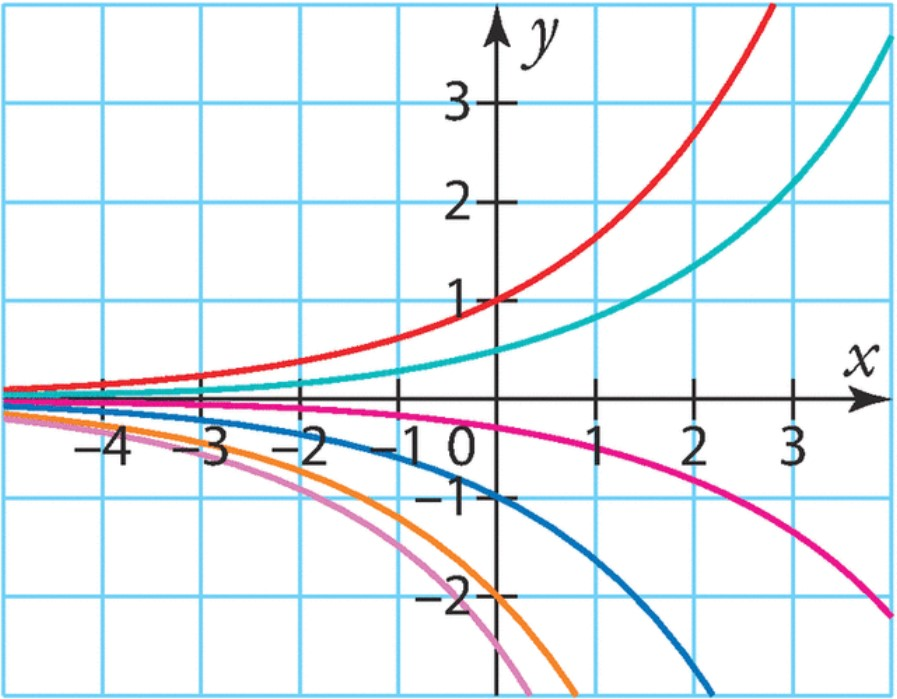
\includegraphics[width=6cm]{courbes2.jpg}}

\textcolor{UGLiBlue}{
    \begin{enumerate}
        \item Soit un point $M_0$ de coordonnées $(x_0\ ;y_0)$.\\
        Les solutions de l'équation différentielle $y'=\dfrac{1}{2}y$ sont les fonctions définies sur $\R$ par $x\mapsto ke^{\frac{1}{2}x}$ où $k$ est une constante réelle.\\
        Donc, pour tout point $M_0$ de coordonnées $(x_0\ ;y_0)$, il existe une unique courbe passant par $M_0$.
        \item Soit $f$ une solution de l'équation différentielle $y'=\dfrac{1}{2}y$ passant par un point $\pc{M_1}{x_1}{2}$.\\
        On a $f(x_1)=2$.\\
        La tangente à la courbe de $f$ au point $M_1$ a pour coefficient directeur $f'(x_1)=\dfrac{1}{2}f(x_1)=\dfrac{1}{2}\times 2=1$.\\
        Or, la droite d'équation $y=x$ a pour coefficient directeur $1$.\\
        La tangente à la courbe de $f$ au point $M_1$ est donc parallèle à la droite d'équation $y=x$.\\
        Donc les tangentes à toutes les courbes au point d'ordonnée $2$ sont parallèles à la droite d'équation $y=x$.
    \end{enumerate}
}

\exo{}
\dleft{11.5cm}{
    Une note de musique est émise en pinçant la corde d'une guitare électrique.    La puissance du son émis, initialement de 100 watts, diminue avec le temps $t$, mesuré en secondes.\\
    On modélise par $f(t)$ la puissance du son émis, exprimée en watts, $t$ secondes après le pincement de la corde. Le son s'affaiblit à une vitesse proportionnelle à sa puissance, il a été établi que le coefficient de proportionnalité est $-0,12$.
}
{
\includegraphics[width=5cm]{guitare.jpg}}
\begin{enumerate}
    \item \faInfo \hspace*{0.1cm} \textit{Si $f$ est la fonction puissance, alors la vitesse d'évolution de cette puissance est $f'$.}\\
    Écrire l'équation différentielle traduisant la diminution de la puissance du son émis.
    \item Déterminer la fonction $f$ solution de cette équation différentielle qui vérifie la condition initiale $f(0)=100$.
    \item Quelle est la puissance du son émis deux secondes après le pincement de la corde ?
    \item Résoudre par le calcul l'équation $f(t)=80$, on donnera la valeur exacte et une valeur approchée à $10^{-3}$ près. Interpréter ce résultat.
\end{enumerate}

\textcolor{UGLiBlue}{
    \begin{enumerate}
        \item L'équation différentielle traduisant la diminution de la puissance du son émis est $f'(t)=-0,12f(t)$.
        \item L'équation différentielle $f'(t)=-0,12f(t)$ est de la forme $y'=ay$ avec $a=-0,12$.\\
        Les solutions de cette équation différentielle sont les fonctions définies sur $\R$ par $t\mapsto ke^{-0,12t}$ où $k$ est une constante réelle.\\
        La fonction $f$ solution de cette équation différentielle qui vérifie la condition initiale $f(0)=100$ est la fonction définie sur $\R$ par $f(t)=100e^{-0,12t}$.
        \item La puissance du son émis deux secondes après le pincement de la corde est 
        \begin{tabbing}
            $f(2)$ \=$=100e^{-0,12\times 2}$\\
            \> $=100e^{-0,24}$\\
            \> $\approx 100\times 0,787$\\
            \> $\approx 78,7$ watts
        \end{tabbing}
        \item \begin{tabbing}
            $f(t)=80$ \= $\iff \quad 100e^{-0,12t}=80$\\
            \> $\iff \quad e^{-0,12t}=\dfrac{80}{100}$\\
            \> $\iff \quad e^{-0,12t}=0,8$\\
            \> $\iff \quad -0,12t=\ln(0,8)$\\
            \> $\iff \quad t=\dfrac{\ln(0,8)}{-0,12}$
        \end{tabbing}
        La solution de l'équation $f(t)=80$ est $\dfrac{\ln(0,8)}{-0,12}$ soit environ $1,860$.\\[.5em]
        Donc la puissance du son émis est de 80 watts environ 1,86 secondes après le pincement de la corde.
    \end{enumerate}
}

\exo{}
\dleft{11.5cm}{
    Une fibre optique est un fil très fin en verre ou en plastique, qui a la propriété de conduire la lumière et sert dans la transmission d'un signal véhiculant des données. La puissance du signal, exprimée en milliwatts (mW), s'atténue au cours de la propagation, exprimée en km.
}
{
\includegraphics[width=5cm]{fiber-optic-2749588_1280.jpg}}
\vspace*{.2cm}

On admet que la fonction puissance $g$ est définie et dérivable sur $\fio{0}{+\infty}$ et qu'elle est solution sur cet intervalle de l'équation différentielle $y'+0,035y=0$.

\begin{enumerate}
    \item Résoudre l'équation différentielle $y'+0,035y=0$.
    \item Sachant que $g(0)=7$, déterminer $g(x)$.
    \item Pour rester détectable, un signal doit être amplifié dès que sa puissance devient inférieure à $0,08$ mW.\\
    Le signal sera-t-il encore detecté au bout de 100 km de propagation ?
\end{enumerate}

\textcolor{UGLiBlue}{
    \begin{enumerate}
        \item L'équation différentielle $y'+0,035y=0$ est de la forme $y'=ay$ avec $a=-0,035$.\\
        Les solutions de cette équation différentielle sont les fonctions définies sur $\R$ par $x\mapsto ke^{-0,035x}$ où $k$ est une constante réelle.
        \item La fonction $g$ solution de cette équation différentielle qui vérifie la condition initiale $g(0)=7$ est la fonction définie sur $\R$ par $g(x)=7e^{-0,035x}$.
        \item La puissance du signal après 100 km de propagation est
        \begin{tabbing}
            $g(100)$ \=$=7e^{-0,035\times 100}$\\
            \> $=7e^{-3,5}$\\
            \> $\approx 7\times 0,0302$\\
            \> $\approx 0,21$ mW
        \end{tabbing}
        Donc le signal sera encore détecté après 100 km de propagation.
    \end{enumerate}
}

\subsection*{Résoudre une équation différentielle de la forme $y'=ay+b$}

\exo{}
Choisir la bonne réponse :
\begin{enumerate}
    \item Une solution particulière de l'équation différentielle $y'+\dfrac{1}{2}y=10$ est :
    \textcolor{UGLiBlue}{
    \begin{multicols}{4}
        \begin{enumerate}[label=]
            \item \ding{51} $20$
            \item \ding{111} $-20$
            \item \ding{111} $10$
            \item \ding{111} $-10$
        \end{enumerate}
    \end{multicols}}

    \item Une solution de l'équation différentielle $y'=2y+2$ est :
    \textcolor{UGLiBlue}{
    \begin{multicols}{2}
        \begin{enumerate}[label=]
            \item \ding{111} $f:x\mapsto e^{-2x}+1$\\[.5em]
            $f'(x)=-2e^{-2x}$\\
            $2f(x)+2=2e^{-2x}+2+2$\\
            $\phantom{2f(x)+2}=2e^{-2x}+4$\\
            $\phantom{2f(x)+2}\neq f'(x)$
            \item \ding{111} $g:x\mapsto e^{-2x}-1$\\[.5em]
            $g'(x)=-2e^{-2x}$\\
            $2g(x)+2=2e^{-2x}-2+2$\\
            $\phantom{2g(x)+2}=2e^{-2x}$\\
            $\phantom{2g(x)+2}\neq g'(x)$
            \item \ding{111} $h:x\mapsto e^{2x}+1$\\[.5em]
            $h'(x)=2e^{2x}$\\
            $2h(x)+2=2e^{2x}+2+2$\\
            $\phantom{2h(x)+2}=2e^{2x}+4$\\
            $\phantom{2h(x)+2}\neq h'(x)$
            \item \ding{51} $k:x\mapsto e^{2x}-1$\\[.5em]
            $k'(x)=2e^{2x}$\\
            $2k(x)+2=2e^{2x}-2+2$\\
            $\phantom{2k(x)+2}=2e^{2x}$\\
            $\phantom{2k(x)+2}=k'(x)$
        \end{enumerate}
    \end{multicols}}
\newpage
    \item La fonction $f$ définie sur $\R$ par $f(x)=2-e^{-4x}$ est solution de l'équation différentielle :\\
    \textcolor{UGLiBlue}{
        On a pour tout $x\in\R, \quad f'(x)=4e^{-4x}$
    \begin{multicols}{2}
        \begin{enumerate}[label=]
            \item \ding{111} $y'-4y=8$\\[.5em]
            $f'(x)-4f(x)=4e^{-4x}-4(2-e^{-4x})$\\
            $\phantom{f'(x)-4f(x)}=4e^{-4x}-8+4e^{-4x}$\\
            $\phantom{f'(x)-4f(x)}=8e^{-4x}-8$
            \item \ding{111} $y'-2y=8$\\[.5em]
            $f'(x)-2f(x)=4e^{-4x}+2(2-e^{-4x})$\\
            $\phantom{f'(x)-2f(x)}=4e^{-4x}+4-2e^{-4x}$\\
            $\phantom{f'(x)-2f(x)}=2e{-4x}+4$
            \item \ding{51} $y'+4y=8$\\[.5em]
            $f'(x)+4f(x)=4e^{-4x}+4(2-e^{-4x})$\\
            $\phantom{f'(x)+4f(x)}=4e^{-4x}+8-4e^{-4x}$\\
            $\phantom{f'(x)+4f(x)}=8$
            \item \ding{111} $y'+2y=8$\\[.5em]
            $f'(x)+2f(x)=4e^{-4x}+2(2-e^{-4x})$\\
            $\phantom{f'(x)+2f(x)}=4e^{-4x}+4-2e^{-4x}$\\
            $\phantom{f'(x)+2f(x)}=2e^{-4x}+4$
        \end{enumerate}
    \end{multicols}}
\end{enumerate}


\exo{}
Résoudre les équations différentielles suivantes :
\begin{multicols}{2}
    \begin{enumerate}
        \item $y'=2y-1$
        \item $y'+2y=3$
    \end{enumerate}
\end{multicols}

\textcolor{UGLiBlue}{
    \begin{enumerate}
        \item L'équation différentielle $y'=2y-1$ est de la forme $y'=ay+b$ avec $a=2$ et $b=-1$.
        \begin{enumerate}[label=\textbullet]
            \item \textbf{Recherche d'une solution particulière constante :}\\
            Soit $y_0$ une solution particulière constante de l'équation différentielle $y'=2y-1$.\\
            On a $y_0'=0$ et $2y_0-1=0$.\\
            Donc $y_0=\dfrac{1}{2}$.
            \item \textbf{Recherche des solutions de l'équation homogène :}\\
            L'équation homogène associée à l'équation différentielle $y'=2y-1$ est $y'=2y$.\\
            Les solutions de cette équation homogène sont les fonctions définies sur $\R$ par $x\mapsto ke^{2x}$ où $k$ est une constante réelle.
            \item \textbf{Conclusion :}\\
            Les solutions de l'équation différentielle $y'=2y-1$ sont les fonctions définies sur $\R$ par $x\mapsto ke^{2x}+ \dfrac{1}{2}$ où $k$ est une constante réelle.
        \end{enumerate}
        \item $y'+2y=3 \quad \iff \quad y'=-2y+3$\\
        L'équation différentielle $y'=-2y+3$ est de la forme $y'=ay+b$ avec $a=-2$ et $b=3$.
        \begin{enumerate}[label=\textbullet]
            \item \textbf{Recherche d'une solution particulière constante :}\\
            Soit $y_0$ une solution particulière constante de l'équation différentielle $y'=-2y+3$.\\
            On a $y_0'=0$ et $-2y_0+3=0$.\\
            Donc $y_0=\dfrac{3}{2}$.
            \item \textbf{Recherche des solutions de l'équation homogène :}\\
            L'équation homogène associée à l'équation différentielle $y'=-2y+3$ est $y'=-2y$.\\
            Les solutions de cette équation homogène sont les fonctions définies sur $\R$ par $x\mapsto ke^{-2x}$ où $k$ est une constante réelle.
            \item \textbf{Conclusion :}\\
            Les solutions de l'équation différentielle $y'+2y=3$ sont les fonctions définies sur $\R$ par $x\mapsto ke^{-2x}+ \dfrac{3}{2}$ où $k$ est une constante réelle.
        \end{enumerate}
    \end{enumerate}
}

\exo{}
\begin{enumerate}
    \item Résoudre $y'-2y=5$.
    \item Déterminer la solution $f$ de cette équation différentielle telle que $f(0)=0$.
\end{enumerate}

\textcolor{UGLiBlue}{
    \begin{enumerate}
        \item $y'-2y=5 \quad \iff \quad y'=2y+5$\\
        L'équation différentielle $y'=2y+5$ est de la forme $y'=ay+b$ avec $a=2$ et $b=5$.
        \begin{enumerate}[label=\textbullet]
            \item \textbf{Recherche d'une solution particulière constante :}\\
            Soit $y_0$ une solution particulière constante de l'équation différentielle $y'=2y+5$.\\
            On a $y_0'=0$ et $2y_0+5=0$.\\
            Donc $y_0=-\dfrac{5}{2}$.
            \item \textbf{Recherche des solutions de l'équation homogène :}\\
            L'équation homogène associée à l'équation différentielle $y'=2y+5$ est $y'=2y$.\\
            Les solutions de cette équation homogène sont les fonctions définies sur $\R$ par $x\mapsto ke^{2x}$ où $k$ est une constante réelle.
            \item \textbf{Conclusion :}\\
            Les solutions de l'équation différentielle $y'-2y=5$ sont les fonctions définies sur $\R$ par $x\mapsto ke^{2x}- \dfrac{5}{2}$ où $k$ est une constante réelle.
            \end{enumerate}
        \item Soit $f$ la solution de cette équation différentielle telle que $f(0)=0$.\\
        On a $f(0)=0 \quad \iff \quad k-\dfrac{5}{2}=0 \quad \iff \quad k=\dfrac{5}{2}$.\\
        Donc la solution de cette équation différentielle telle que $f(0)=0$ est la fonction définie sur $\R$ par $f(x)=\dfrac{5}{2}e^{2x}- \dfrac{5}{2}$.
    \end{enumerate}
}

\exo{}
On considère l'équation différentielle $(E) : y'-5y=3$.
\begin{enumerate}
    \item Résoudre l'équation différentielle $(E)$.
    \item Déterminer la solution $f$ de $(E)$ telle que $f(0)=\dfrac{-6}{5}$.
    \item Étudier les variations de la fonction $f$ sur $\R$.
    \item Déterminer les limites de $f$ en $+\infty$ et $-\infty$.
    \item Déterminer la valeur de $x$ pour laquelle $f(x)=-10$.
\end{enumerate}

\textcolor{UGLiBlue}{
    \begin{enumerate}
        \item $y'-5y=3 \quad \iff \quad y'=5y+3$\\
        L'équation différentielle $y'=5y+3$ est de la forme $y'=ay+b$ avec $a=5$ et $b=3$.
        \begin{enumerate}[label=\textbullet]
            \item \textbf{Recherche d'une solution particulière constante :}\\
            Soit $y_0$ une solution particulière constante de l'équation différentielle $y'=5y+3$.\\
            On a $y_0'=0$ et $5y_0+3=0$.\\
            Donc $y_0=-\dfrac{3}{5}$.
            \item \textbf{Recherche des solutions de l'équation homogène :}\\
            L'équation homogène associée à l'équation différentielle $y'=5y+3$ est $y'=5y$.\\
            Les solutions de cette équation homogène sont les fonctions définies sur $\R$ par $x\mapsto ke^{5x}$ où $k$ est une constante réelle.
            \item \textbf{Conclusion :}\\
            Les solutions de l'équation différentielle $y'-5y=3$ sont les fonctions définies sur $\R$ par $x\mapsto ke^{5x}- \dfrac{3}{5}$ où $k$ est une constante réelle.
        \end{enumerate}
        \item Soit $f$ la solution de cette équation différentielle telle que $f(0)=-\dfrac{6}{5}$.
        \begin{tabbing}
            On a : $f(0)=-\dfrac{6}{5} \quad$ \=$\iff \quad k-\dfrac{3}{5}=-\dfrac{6}{5}$\\[.5em]
            \> $\iff \quad k=-\dfrac{6}{5}+\dfrac{3}{5}$\\[.5em]
            \> $\iff \quad k=-\dfrac{3}{5}$
        \end{tabbing}
        Donc la solution de cette équation différentielle telle que $f(0)=-\dfrac{6}{5}$ est la fonction définie sur $\R$ par $f(x)=-\dfrac{3}{5}e^{5x}- \dfrac{3}{5}$.
        \item $f'(x)=5(-\dfrac{3}{5}e^{5x})= -3e^{5x}<0$.\\[.5em]
        Donc $f$ est décroissante sur $\R$.
        \item $\lim\limits_{x\to +\infty}f(x)=\lim\limits_{x\to +\infty}-\dfrac{3}{5}e^{5x}- \dfrac{3}{5}=« -\dfrac{3}{5}\times (+\infty)- \dfrac{3}{5} »=-\infty$.\\[.5em]
        $\lim\limits_{x\to -\infty}f(x)=\lim\limits_{x\to -\infty}-\dfrac{3}{5}e^{5x}- \dfrac{3}{5}=« -\dfrac{3}{5}\times 0- \dfrac{3}{5}»=- \dfrac{3}{5}$.
        \item \begin{tabbing}
            $f(x)=-10$ \= $\iff \quad -\dfrac{3}{5}e^{5x}- \dfrac{3}{5}=-10$\\[.5em]
            \> $\iff \quad -\dfrac{3}{5}e^{5x}=-10+\dfrac{3}{5}$\\[.5em]
            \> $\iff \quad -\dfrac{3}{5}e^{5x}=\dfrac{3}{5}-\dfrac{50}{5}$\\[.5em]
            \> $\iff \quad -\dfrac{3}{5}e^{5x}=-\dfrac{47}{5}$\\[.5em]
            \> $\iff \quad e^{5x}=\dfrac{47}{3}$\\[.5em]
            \> $\iff \quad 5x=\ln\left(\dfrac{47}{3}\right)$\\[.5em]
            \> $\iff \quad x=\dfrac{\ln\left(\dfrac{47}{3}\right)}{5}$
        \end{tabbing}
    \end{enumerate}
}

\exo{ Décharge d'un condensateur physique}
\dleft{12cm}{
    Un condensateur de capacité $C$ farads est chargé sous une tension initiale de 20 volts. Il se décharge ensuite dans une résistance de $R$ ohms.\\
    En notant $u(t)$ la tension (en volts) aux bornes du condensateur au bout de $t$ secondes, $u$ est alors une fonction définie sur $\fio{0}{+\infty}$ qui est solution de l'équation différentielle $y'+\dfrac{1}{RC}y=0$.
}
{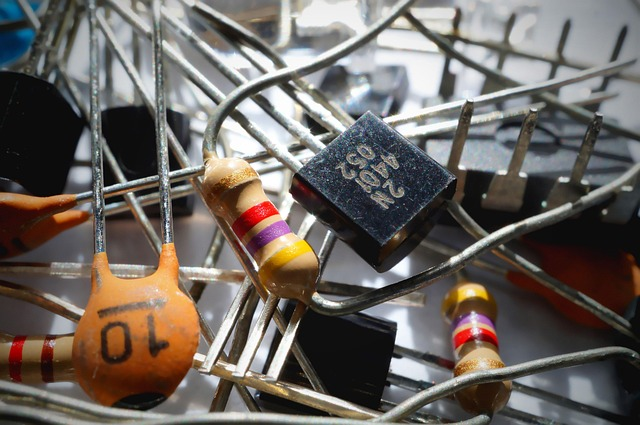
\includegraphics[width=4.5cm]{capacitor-1835729_640.jpg}}
\begin{enumerate}
    \item Résoudre l'équation différentielle $y'+\dfrac{1}{RC}y=0$ et en déduire l'expression de la fonction $u$.
    \item On suppose que $R=1000$ et $C=10^{-4}$.\\
    Pendant combien de temps (au centième de seconde près) la tension aux bornes du condensateur reste-t-elle supérieure ou égale à 5 volts ?
\end{enumerate}

\textcolor{UGLiBlue}{
    \begin{enumerate}
        \item $y'+\dfrac{1}{RC}y=0 \quad \iff \quad y'=-\dfrac{1}{RC}y$\\[.5em]
        L'équation différentielle $y'=-\dfrac{1}{RC}y$ est de la forme $y'=ay$ avec $a=-\dfrac{1}{RC}$.\\
        Les solutions de cette équation différentielle sont les fonctions définies sur $\R$ par $t\mapsto ke^{-\frac{1}{RC}t}$ où $k$ est une constante réelle.\\
        La fonction $u$ est définie sur $\R$ par $t\mapsto ke^{-\frac{1}{RC}t}$ où $k$ est une constante réelle.\\
        On a $u(0)=20$ donc $k=20$.\\
        Donc la fonction $u$ est définie sur $\R$ par $u(t)= 20e^{-\frac{1}{RC}t}$.
        \item On a $u(t)=20e^{-\frac{1}{RC}t}=20e^{-\frac{1}{1000\times 10^{-4}}t}=20e^{-10t}$.
        \begin{tabbing}
            $u(t)\geqslant 5 \quad$ \= $\iff \quad 20e^{-10t}\geqslant 5$\\
            \> $\iff \quad e^{-10t}\geqslant \dfrac{5}{20}$\\
            \> $\iff \quad e^{-10t}\geqslant \dfrac{1}{4}$\\[.5em]
            \> $\iff \quad -10t\geqslant \ln\left(\dfrac{1}{4}\right)$\\[.5em]
            \> $\iff \quad t\leqslant \dfrac{\ln\left(\dfrac{1}{4}\right)}{-10}$\\[.5em]
            \> $\iff \quad t\leqslant \dfrac{\ln(4)}{10}$
        \end{tabbing}
    \end{enumerate}
}

\newpage
\exo{ Loi de refroidissement de Newton}
Un corps est placé dans une enceinte dont on maintient la température constante égale à 20°C. À l'instant initial $t=0$, la température du corps est de 70°C et, après 5 min, elle n'est plus que de 60°C.\\
La température du corps en fonction du temps (en min) est notée $T(t)$. $T$ est une fonction définie sur $\fio{0}{+\infty}$. La loi de refroidissement de Newton énonce que $T'$ est propotionnelle à $T-20$.
\begin{enumerate}
    \item Justifier que la fonction $t\mapsto T(t)-20$ est solution d'une équation différentielle de la forme $y'=ay$, puis déterminer la fonction $T$.
    \item Déterminer la température du corps (au degré près) après une demi-heure.
    \item Après combien de temps (à la minute près) la température du corps sera-t-elle de 40°C ?
\end{enumerate}

\textcolor{UGLiBlue}{
    \begin{enumerate}
        \item $T'(t)$ est proportionnelle à $T(t)-20$ donc $T'(t)=a(T(t)-20)$ où $a$ est une constante réelle.\\
        Soit $f:t\mapsto T(t)-20$.\\
        On a $f'(t)=T'(t)$ et $f(t)=T(t)-20$.\\
        Donc $f'(t)=af(t)$.\\[1em]
        Les solutions de cette équation différentielle sont les fonctions définies sur $\R$ par $t\mapsto ke^{at}$ où $k$ est une constante réelle.\\
        Donc $f(t)=ke^{at}$ et $T(t)=20+ke^{at}$.\\
        On a $T(0)=70$ donc $20+k=70$ et $k=50$.\\
        On a $T(5)=60$ donc $20+50e^{5a}=60$ et $e^{5a}=\dfrac{40}{50}=\dfrac{4}{5}=0,8$.\\
        Donc $5a=\ln(0,8)$ et $a=\dfrac{\ln(0,8)}{5}$.\\
        Donc $T(t)=20+50e^{\frac{\ln(0,8)}{5}t}$.
        \item \begin{tabbing}
            $T(30)$ \=$=20+50e^{\frac{\ln(0,8)}{5}\times 30}$\\
            \> $=20+50e^{6\ln(0,8)}$\\
            \> $=20+50\times 0,8^6$\\
            \> $\approx 20+50\times 0,262$\\
            \> $\approx 20+13,1$\\
            \> $\approx 33,1$
        \end{tabbing}
        Après une demi-heure, la température du corps est d'environ 33°C.
        \item \begin{tabbing}
            $T(t)=40$ \= $\iff \quad 20+50e^{\frac{\ln(0,8)}{5}t}=40$\\
            \> $\iff \quad 50e^{\frac{\ln(0,8)}{5}t}=20$\\
            \> $\iff \quad e^{\frac{\ln(0,8)}{5}t}=\dfrac{20}{50}$\\
            \> $\iff \quad e^{\frac{\ln(0,8)}{5}t}=\dfrac{2}{5}$\\
            \> $\iff \quad \dfrac{\ln(0,8)}{5}t=\ln\left(\dfrac{2}{5}\right)$\\
            \> $\iff \quad t=\dfrac{5\ln\left(\dfrac{2}{5}\right)}{\ln(0,8)}$
        \end{tabbing}
        Or $\dfrac{5\ln\left(\dfrac{2}{5}\right)}{\ln(0,8)}\approx 20,53$.\\
        Donc la température du corps sera de 40°C environ 21 minutes après le début de l'expérience.
    \end{enumerate}
}

%\newpage
\exo{ Croissance de bactéries}
La nombre de bactéries $B$ d'une culture passe de 600 à l'instant initial à 1800 après 2 heures. On suppose que le taux de croissance est directement proportionnel au nombre de bactéries présentes.\\[.5em]
Déterminer :
\begin{enumerate}
        \item Une équation avec des conditions qui traduisent le problème.
        \item Une formule qui permet de calculer le nombre de bactéries $B(t)$ à l'instant $t$.
        \item Le nombre de bactéries après 4 heures.
        \item Le temps nécessaire pour que le nombre de bactéries dépasse 12 000.
\end{enumerate}

\textcolor{UGLiBlue}{
    \begin{enumerate}
        \item Soit $B(t)$ le nombre de bactéries après $t$ heures de culture.\\
        On a $B(0)=600$ et $B(2)=1800$.\\
        $B'(t)$ est proportionnel à $B(t)$ donc $B'(t)=aB(t)$ où $a$ est une constante réelle.\\
        $B$ est donc solution de l'équation différentielle $y'=ay$ et vérifie les conditions $B(0)=600$ et $B(2)=1800$.
        \item Les solutions de l'équation différentielle $y'=ay$ sont les fonctions définies sur $\R$ par $t\mapsto ke^{at}$ où $k$ est une constante réelle.\\
        Il existe donc une constante $k$ telle que $B(t)=ke^{at}$. Or $B(0)=600$ donc $k=600$.\\
        Ainsi $B(t)=600e^{at}$.
        \begin{tabbing}
            $B(2)=1800 \quad$ \= $\iff \quad 600e^{2a}=1800$\\
            \> $\iff \quad e^{2a}=\dfrac{1800}{600}$\\
            \> $\iff \quad e^{2a}=3$\\
            \> $\iff \quad 2a=\ln(3)$\\
            \> $\iff \quad a=\dfrac{\ln(3)}{2}$
        \end{tabbing}
        Ainsi $B(t)=600e^{\frac{\ln(3)}{2}t}$.
        \item \begin{tabbing}
            $B(4)$ \= $=600e^{\frac{\ln(3)}{2}\times 4}$\\
            \> $=600e^{2\ln(3)}$\\
            \> $=600\times 3^2$\\
            \> $=600\times 9$\\
            \> $=5400$
        \end{tabbing}
        Le nombre de bactéries après 4 heures est de 5400.
        \item \begin{tabbing}
            $B(t)>12000$ \= $\iff \quad 600e^{\frac{\ln(3)}{2}t}>12000$\\
            \> $\iff \quad e^{\frac{\ln(3)}{2}t}>20$\\
            \> $\iff \quad \dfrac{\ln(3)}{2}t>\ln(20)$\\
            \> $\iff \quad t>\dfrac{2\ln(20)}{\ln(3)} \qquad$ car $\dfrac{\ln(3)}{2}>0$\\
        \end{tabbing}
        Or $\dfrac{2\ln(20)}{\ln(3)}\approx 5,45$.\\
        Donc le nombre de bactéries dépasse 12 000 après environ 5,5 heures.
    \end{enumerate}
}

\exo{ En économie}
Dans une économie keynésienne simple, la consommation $C$ s'exprime par l'égalité $C=360+0,8Y$ et $I=120$, où $Y$ est le revenu et $I$ l'investissement.\\
Lorsque le marché est hors de l'équilibre, on suppose que le revenu $Y$ évolue en fonction du temps selon l'équation différentielle $Y'=0,25(C+I-Y)$.\\
À la période initiale, le revenu $Y_0$ est égal à 2000.
\begin{enumerate}
    \item Écrire l'équation différentielle vérfiée par la fonction $Y$.
    \item Déterminer la fonction $Y$.
    \item Étudier la limite de la fonction $Y$ en $+\infty$ et en déduire une conclusion sur la stabilité de l'équilibre de cette économie.
\end{enumerate}

\textcolor{UGLiBlue}{
    \begin{enumerate} 
        \item \begin{tabbing}
            $Y'=0,25(C+I-Y) \quad$ \= $\iff \quad Y'=0,25(360+0,8Y+120-Y)$\\
        \> $\iff \quad Y'=0,25(480+0,8Y-Y)$\\
        \> $\iff \quad Y'=0,25(480-0,2Y)$\\
        \> $\iff \quad Y'=120-0,05Y$
    \end{tabbing}
        \item $Y$ est solution de l'équation différentielle $y'=0,05y+120$.\\
        \begin{enumerate}
            \item \textbf{Recherche d'une solution particulière constante :}\\
            Soit $y_0$ une solution particulière constante de l'équation différentielle $y'=0,05y+120$.\\
            On a $y_0'=0$ et $0,05y_0+120=0$.\\
            Donc $y_0=-2400$.
            \item \textbf{Recherche des solutions de l'équation homogène :}\\
            L'équation homogène associée à l'équation différentielle $y'=0,05y+120$ est $y'=0,05y$.\\
            Les solutions de cette équation homogène sont les fonctions définies sur $\R$ par $x\mapsto ke^{0,05x}$ où $k$ est une constante réelle.
            \item \textbf{Conclusion :}\\
            Les solutions de l'équation différentielle $y'=0,05y+120$ sont les fonctions définies sur $\R$ par $x\mapsto ke^{0,05x}-2400$ où $k$ est une constante réelle.\\
            Donc il existe une constante $k$ telle que $Y(t)=ke^{0,05t}-2400$.\\
            \item \textbf{Condition initiale :}
            \begin{tabbing}
                $Y(0)=2000$ \= $\iff \quad k-2400=2000$\\
                \> $\iff \quad k=4400$
            \end{tabbing}
            On a donc $Y(t)=4400e^{0,05t}-2400$.
        \end{enumerate}
        \item \begin{tabbing}
            $\lim\limits_{t\to +\infty}Y(t)$ \= $=\lim\limits_{t\to +\infty}4400e^{0,05t}-2400$\\
            \> $=« 4400\times +\infty-2400 »$\\
            \> $=+\infty$
        \end{tabbing}
        Donc le revenu de cette économie tend vers l'infini.\\
        L'équilibre de cette économie n'est pas stable.
    \end{enumerate}
}
\end{document}